% Focal Loss Curve Diagram
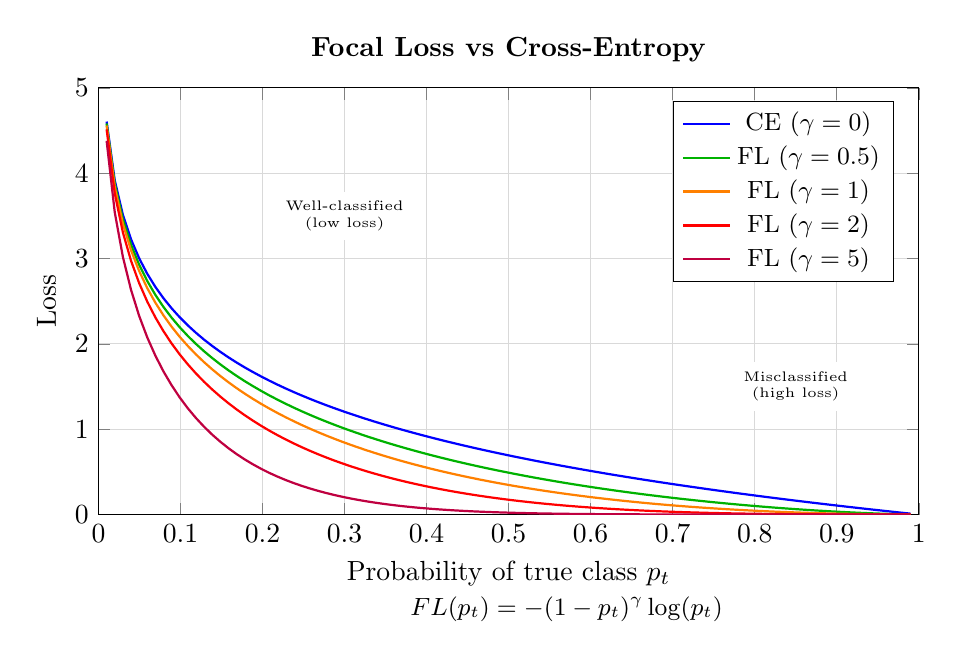
\begin{tikzpicture}
\begin{axis}[
    width=12cm,
    height=7cm,
    xlabel={Probability of true class $p_t$},
    ylabel={Loss},
    xmin=0, xmax=1,
    ymin=0, ymax=5,
    legend pos=north east,
    legend style={font=\small},
    grid=major,
    grid style={gray!30},
    title={\textbf{Focal Loss vs Cross-Entropy}},
    title style={font=\bfseries}
]

% Cross-Entropy (gamma = 0)
\addplot[
    domain=0.01:0.99,
    samples=100,
    thick,
    blue
] {-ln(x)};
\addlegendentry{CE ($\gamma=0$)}

% Focal Loss gamma = 0.5
\addplot[
    domain=0.01:0.99,
    samples=100,
    thick,
    green!70!black
] {-(1-x)^0.5 * ln(x)};
\addlegendentry{FL ($\gamma=0.5$)}

% Focal Loss gamma = 1
\addplot[
    domain=0.01:0.99,
    samples=100,
    thick,
    orange
] {-(1-x)^1 * ln(x)};
\addlegendentry{FL ($\gamma=1$)}

% Focal Loss gamma = 2
\addplot[
    domain=0.01:0.99,
    samples=100,
    thick,
    red
] {-(1-x)^2 * ln(x)};
\addlegendentry{FL ($\gamma=2$)}

% Focal Loss gamma = 5
\addplot[
    domain=0.01:0.99,
    samples=100,
    thick,
    purple
] {-(1-x)^5 * ln(x)};
\addlegendentry{FL ($\gamma=5$)}

% Annotation
\node[align=center, font=\tiny, fill=white] at (axis cs:0.3, 3.5) {
    Well-classified\\
    (low loss)
};

\node[align=center, font=\tiny, fill=white] at (axis cs:0.85, 1.5) {
    Misclassified\\
    (high loss)
};

\end{axis}

% Formula
\node[font=\small, align=center] at (6, -1.2) {
    $\text{FL}(p_t) = -(1-p_t)^\gamma \log(p_t)$
};

\end{tikzpicture}




